\documentclass[english]{article}

\usepackage{babel}
\usepackage{graphicx}
\usepackage{alltt}
\usepackage{url}
\usepackage{tabularx}
%\usepackage{ngerman}
\usepackage{longtable}
\usepackage{color}
\usepackage{framed}

\usepackage{xifthen}
\newboolean{showbackdoors}
\setboolean{showbackdoors}{true}  % set to false to hide subsection on backdoors for reviewing group


\newenvironment{prettytablex}[1]{\vspace{0.3cm}\noindent\tabularx{\linewidth}{@{\hspace{\parindent}}#1@{}}}{\endtabularx\vspace{0.3cm}}
%\newenvironment{prettytable}{\prettytablex{l X}}{\endprettytablex}



\title{\huge\sffamily\bfseries System Description and Risk Analysis}
\author{B\"ahler Alessio \and Enz Andreas \and Niederberger Matthias}
\date{\today}


\begin{document}
\maketitle

%% **** please observe the page limit **** 
%% (it is not allowed to change the font size or page geometry to gain more space)
%% comment or remove lines below before hand-in

%%%%%%%%%%%%%%%%%%%%%%%%%%%%%%%%%%%%%%%%%%%%%%

\tableofcontents
\pagebreak


\section{System Characterization}

\subsection{System Overview}


%%% Describe the system's mission,  the system boundaries,
%%% and the overall system architecture, including the main subsystems and
%%% their relationships.   This description should provide a high-level
%%% overview of the system, e.g., suitable for managers, that complements
%%% the more technical description that follows.


The System consists of three machines in a company network and external client machines that connect over the Internet. Inside the company network we have Machine 1 housing the Core CA functionality and the legacy MySQL database. Machine 2 contains the web server with a firewall to shield it because any traffic from outside the company network will have to cross the web server machine anyway. Finally Machine 3 is used for the physical separation of the backup service, with backup daemons connecting to the other two machines.



\begin{figure}[htb!]
\centering{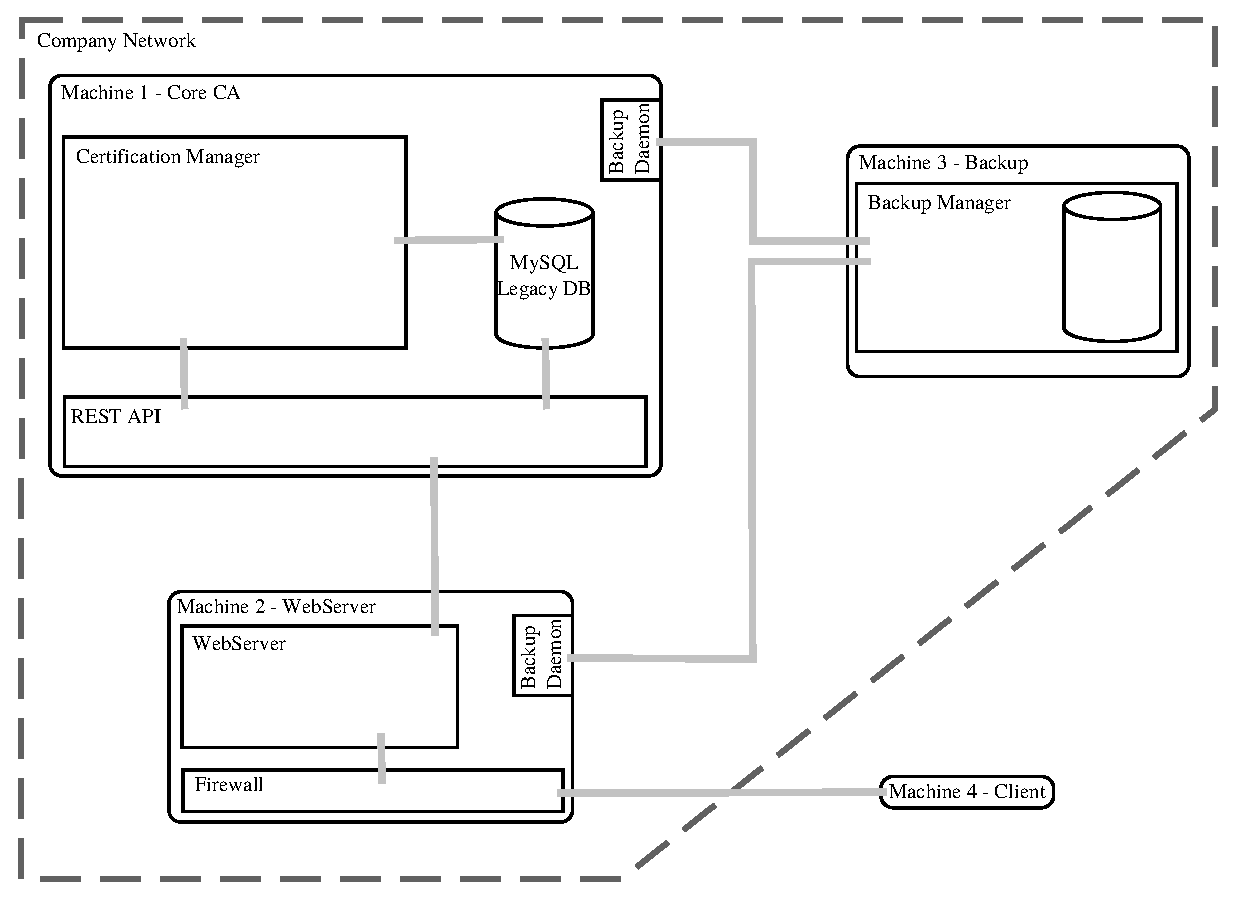
\includegraphics[width=\textwidth]{res/system_arch.eps}}
\caption{System Architecture of the company network including an external client machien.}
\centering
\label{fig:system_arch}
\end{figure}


\subsection{Components}

%%% List all system components and their interfaces, subdivided, for example, into
%%%   categories such as platforms, applications, data records, etc. For
%%%   each component, state its relevant properties.

A short description of the components in Figure \ref{fig:system_arch}.

\begin{itemize}
    \item \textbf{Certification Manager}: Manages certificate state (creation, revocation, deletion, ...). Interfaces with the web server over the REST API and directly with the legacy MySQL database. It has two main subcomponents: 
    \begin{itemize}
        \item Certification Store: A directory where keys and certificates are stored.
        \item Certification Generator: Built with OpenSSL
    \end{itemize}
    \item \textbf{MySQL DB}: As provided. Interfaces with the web server over a REST AP and with the Certification Manager.
    \item \textbf{REST API}: Interface between Core CA machine and WebServer machine.
    \item \textbf{Web Server}: Accepts web traffic filtered through a Firewall. Does Authorization by checking legacy database and can request certificate state changes from the Certification Manager.
    \item \textbf{Firewall}: Filters traffic.
    \item \textbf{Backup Manager}: Periodically stores specified data in the backup database. Interfaces with Core CA and WebServer machine.
    \begin{itemize}
        \item Backup Daemon: Sends Data to Backup machine
    \end{itemize}
\end{itemize}



\section{Risk Analysis and Security Measures}

\subsection{Assets}

%% TODO: Describe the relevant assets and their required security
%%  properties. For example, data objects, access restrictions,
%%  configurations, etc.
 
\textbf{Physical Assets}
\begin{itemize}
\item Web Server: physical machine hosting the Web Server Application
\item Core CA: physical machine hosting the CA Application and the legacy database
\item Backup: physical machine hosting the backup data
\end{itemize}

\textbf{Logical Assets}
\begin{itemize}
\item Software
\begin{itemize}
\item Web Server Application
\item Core CA Application
\item legacy MySQL database/application/driver?
\item REST API
\item Backup Daemon
\item Backup Manager
\item Firewall
\end{itemize}
\item Information
\begin{itemize}
\item Certificates
\item Keys
\item User data
\item Configuration files
\item Logs
\end{itemize}
\end{itemize}

\textbf{Persons}
\begin{itemize}
\item System Administrator: maintains the system by applying software updates, controlling system's logs to search malicious behaviours that could lead to security issues and ensuring that the machines hosting the system's components are working properly. He therefore has access to sensitive data, in the form of a remote connection well as to physical access to all components.
\item CA Administrators: are able to verify the current state of the CA 
\item Users: Employees and Informants: both use the system to obtain certificates that allows them to communicate securely.
\item Management
\end{itemize}

\textbf{Intangible Goods}
\begin{itemize}
\item Company Reputation
\end{itemize}

\subsection{Threat Sources}

TODO: Name and describe potential threat sources (\emph{not} threats!) including their motivation.

\begin{itemize}
\item Nature: probably not relevant since it targets availability
\item Users: Employees (includes also cleaning personnel etc.) and Informants can act maliciously or be careless/poorly trained
\item Competitors: may be interested in obtaining confidential information to gain an advantage, blackmail or cause harm by publishing it. May resort to Skilled Hackers to achieve their goals.
\item "Victims": subjects of investigative reports that were publicly exposed and may want to get revenge by causing any kind of damage. May resort to Skilled Hackers to achieve their goals.
\item Organized Crime: can directly or indirectly be "Victim", could be interested in blackmailing the Company to gain money or just to obtain important information that can be sold on the black market/used for other illegal activities.
\item Malware: TODO
\item Expert Hackers: A skilled hacker has expert knowledge for some systems. He can write his own code and may use unknown or unpublished vulnerabilities (from book). May itself be a "Victim" or act for monetary interests.
\item Script Kiddies: This type of adversary has basic computer knowledge and uses mainly known vulnerabilities for which exploits are available on the Internet. However, he might write scripts to automate tasks or use tools to automatically create malware. His main motivations are challenge, glory and destruction (from book).
\item Organizatorial Deficiencies (from SecEng slides): lack in employee training, poor/non-existing/non-enforced security measures (E.g. TODO) can weaken the overall security of the system.
\item Hardware Failures (from SecEng slides): TODO
\end{itemize}

\subsection{Risks Definitions}

Define likelihood, impact and risk level using the following three
  tables \cite{ASL_book}.

%\subsubsection{Tools}

\begin{center}
\begin{tabular}{|l|p{0.8\textwidth}|}
\hline
%\multicolumn{2}{|c|}{\bf Likelihood} \\
%\hline
Likelihood & Description \\
\hline
\hline
High   & The threat source is highly motivated and sufficiently capable of exploiting a given vulnerability in order to change the asset's state. The controls to prevent the vulnerability from being exploited are ineffective. \\
\hline
Medium & The threat source is motivated and capable of exploiting a given vulnerability in order to change the asset's state, but controls are in place that may impede a successful exploit of the vulnerability. \\
\hline
Low   & The threat source lacks motivation or capabilities to exploit a given vulnerability in order to change the asset's state. Another possibility that results in a low likelihood is the case where controls are in place that prevent (or at least significantly impede) the vulnerability from being exercised. \\
\hline
\end{tabular}
\hspace{3em}
\begin{tabular}{|l|p{0.8\textwidth}|}
\hline
\multicolumn{2}{|c|}{\bf Impact} \\
\hline
Impact & Description \\
\hline
\hline
High   & The event (1) may result in a highly costly loss of major tangible assets or resources; (2) may significantly violate, harm, or impede an organization's mission, reputation, or interest; or (3) may result in human death or serious injury. \\
\hline
Medium & The event (1) may result in a costly loss of tangible assets or resources; (2) may violate, harm, or impede an organization's mission, reputation, or interest, or (3) may result in human injury. \\
\hline
Low   & The event (1) may result in a loss of some tangible assets or resources or (2) may noticeably affect an organization's mission, reputation, or inter- est. \\
\hline
\end{tabular}
\end{center}

\vspace{5mm}

\begin{center}
\begin{tabular}{|l|c|c|c|}
\hline
\multicolumn{4}{|c|}{{\bf Risk Level}} \\
\hline
{{\bf Likelihood}} & \multicolumn{3}{c|}{{\bf Impact}} \\ %\cline{2-4}
     & Low & Medium & High \\  \hline
 High & Low & Medium & High  \\
\hline
 Medium & Low & Medium & Medium \\
\hline
 Low & Low & Low & Low \\
\hline
\end{tabular}
\end{center}


\subsection{Risk Evaluation}

List all potential threats and the corresponding countermeasures. Estimate the risk based on the information about the threat, the threat sources and the corresponding countermeasure. Adhere to the risk definitions you have given above. As a sanity check, there should be at least one high-risk entry.


\subsubsection{{\it Evaluation Web Server}}

Evaluate the likelihood, impact and the resulting risk,  \emph{after implementation of the corresponding countermeasures}. Formulate the threats in active, not passive, 
voice: who (threat source) does what (threat action)? 

\begin{footnotesize}
\begin{prettytablex}{llp{5.5cm}lll}
No. & Threat &  Countermeasure(s) & L & I & Risk \\
\hline
1 & Exper Hackers: mount an active  & ... & {\it Low} & {\it Low} & {\it Low} \\
\hline
2 & ... & ...& {\it Medium} & {\it High} & {\it Medium} \\
\hline
\end{prettytablex}
\end{footnotesize}

\subsubsection{{\it Evaluation Backup}}

Evaluate the likelihood, impact and the resulting risk,  \emph{after implementation of the corresponding countermeasures}. Formulate the threats in active, not passive, 
voice: who (threat source) does what (threat action)? 

\begin{footnotesize}
\begin{prettytablex}{llp{5.5cm}lll}
No. & Threat &  Countermeasure(s) & L & I & Risk \\
\hline
1 & Hardware failure & ... & {\it Low} & {\it Low} & {\it Low} \\
\hline
2 & ... & ...& {\it Medium} & {\it High} & {\it Medium} \\
\hline
\end{prettytablex}
\end{footnotesize}

\subsubsection{{\it Evaluation Users}}

Evaluate the likelihood, impact and the resulting risk,  \emph{after implementation of the corresponding countermeasures}. Formulate the threats in active, not passive, 
voice: who (threat source) does what (threat action)? 

\begin{footnotesize}
\begin{prettytablex}{llp{5.5cm}lll}
No. & Threat &  Countermeasure(s) & L & I & Risk \\
\hline
1 &  & ... & {\it Low} & {\it Low} & {\it Low} \\
\hline
2 & ... & ...& {\it Medium} & {\it High} & {\it Medium} \\
\hline
\end{prettytablex}
\end{footnotesize}

\subsubsection{{\it Evaluation Asset y}}

\begin{footnotesize}
\begin{prettytablex}{llp{5.5cm}lll}
No. & Threat & Countermeasure(s) & L & I & Risk \\
\hline
1 & ... & ... & {\it Low} & {\it Low} & {\it Low} \\
\hline
2 & ... & ...& {\it Medium} & {\it High} & {\it Medium} \\
\hline
\end{prettytablex}
\end{footnotesize}

\subsubsection{Detailed Description of Selected Countermeasures}

Optionally explain the details of the countermeasures mentioned above.



\subsubsection{Risk Acceptance}

List all medium and high risks, according to the evaluation above. For each risk, propose additional countermeasures that could be implemented to further reduce the risks.

\begin{footnotesize}
\begin{prettytablex}{p{2cm}X}
No. of threat & Proposed additional countermeasure including expected impact  \\
\hline
... & ... \\
\hline
... & ... \\
\hline
\end{prettytablex}
\end{footnotesize}

\begin{thebibliography}{---}
\bibitem[1]{ASL_book} Computer Security: Principles and Practice. William Stallings and Laurie Brown, Prentice Hall, 2008 
Applied Information Security: A Hands-on Approach, David Basin, Patrick Schaller and Michael Schl�pfer, Springer, 2011
\end{thebibliography}

\end{document}

%%% Local Variables: 
%%% mode: latex
%%% TeX-master: "../../book"
%%% End: 
